% !TeX -lualatex 
\documentclass[ba,logo]{ivs-thesis} 

%%%%%%%%%%%%%%%%%%%%%%%%%%%%%%%%%%%
% Language Settings
%%%%%%%%%%%%%%%%%%%%%%%%%%%%%%%%%%%

% To specify the language of your thesis, uncomment the appropriate setting
% which depends on your LaTeX compiler. If you use a modern compiler such as
% LuaLaTeX or XeLaTeX, it is recommended to use the 'polyglossia' package to
% specify the language. If you use LaTeX or PDFLaTeX, 'babel' is recommended. 

% English

% LuaLaTeX or XeLaTeX 
\usepackage{polyglossia}
\setmainlanguage{english} 

% PDFLaTeX 
%\usepackage[english]{babel}

% German 

% LuaLaTeX or XeLaTeX 
%\usepackage{polyglossia}
%\setmainlanguage{german} 

% PDFLaTeX 
%\usepackage[ngerman]{babel}

\usepackage{algorithm}
\usepackage[noend]{algpseudocode}

%%%%%%%%%%%%%%%%%%%%%%%%%%%%%%%%%%%
% Settings for list environments 
%%%%%%%%%%%%%%%%%%%%%%%%%%%%%%%%%%%

\usepackage{enumitem}

\setlist{nosep,topsep=1ex,labelindent=\parindent,listparindent=\parindent}

\setlist[description]{leftmargin=2cm,style=nextline}

\setlist[enumerate,1]{label=(\roman*)}
\setlist[enumerate,2]{label=(\alph*)}
\setlist[enumerate,3]{label=(\arabic*)} 

\setlist[itemize,1]{label=\textbullet}
\setlist[itemize,2]{label=\rule[.2ex]{0.8ex}{0.8ex}}
\setlist[itemize,3]{label=-}

%%%%%%%%%%%%%%%%%%%%%%%%%%%%%%%%%%%
% Useful Packages and Settings 
%%%%%%%%%%%%%%%%%%%%%%%%%%%%%%%%%%%

\usepackage{csquotes} 
\usepackage{amssymb}
\usepackage{amsmath}
\usepackage{hyperref}
\usepackage{tabularx}

%%%%%%%%%%%%%%%%%%%%%%%%%%%%%%%%%%%
% Demo Packages
%%%%%%%%%%%%%%%%%%%%%%%%%%%%%%%%%%%

% The packages included and settings set here are solely for the demo document
% and can be removed in your thesis 

\usepackage{metalogo} 
\usepackage{fancyvrb}

\RecustomVerbatimEnvironment{Verbatim}{Verbatim}{xleftmargin=\parindent,numbers=left,firstnumber=last,tabsize=4} 

%%%%%%%%%%%%%%%%%%%%%%%%%%%%%%%%%%%
% Citation Package
%%%%%%%%%%%%%%%%%%%%%%%%%%%%%%%%%%%
\usepackage{varioref}
\usepackage{cleveref}
\usepackage[backend=biber,style=authoryear]{biblatex}
\renewcommand*{\nameyeardelim}{\addcomma\space} 


%%%%%%%%%%%%%%%%%%%%%%%%%%%%%%%%%%%%
% Theoremstyles
%%%%%%%%%%%%%%%%%%%%%%%%%%%%%%%%%%%%
\theoremstyle{break}
\theorembodyfont{\normalfont}
\theoremseparator{.}
\theorempreskip{1em}
\theorempostskip{1em}
\theoremsymbol{\ensuremath{\diamond}}

\newtheorem{thm}{Theorem}[chapter]
\newtheorem{lem}[thm]{Lemma}
\newtheorem{prop}[thm]{Proposition}
\newtheorem{cor}[thm]{Corollary}

\newtheorem{exa}[thm]{Example}
\newtheorem{exas}[thm]{Examples}

\newtheorem{prblm}[thm]{Problem}
\newtheorem{prblms}[thm]{Problems}

\newtheorem{quest}{Question}
\newtheorem{quests}{Questions}

\newtheorem{rmk}[thm]{Remark}
\newtheorem{rmks}[thm]{Remarks}

\newtheorem{defn}[thm]{Definition}

\theoremstyle{nonumberplain}
\theoremheaderfont{\itshape}
\theoremsymbol{\rule{1ex}{1ex}}

\newtheorem{proof}{Proof}

\newcommand{\x}{\boldsymbol{x}}
\newcommand{\y}{\boldsymbol{y}}
\newcommand{\vp}{\boldsymbol{v}^+}
\newcommand{\vm}{\boldsymbol{v}^-}
\newcommand{\ve}{\boldsymbol{v}} 

\title{Unpaired Image Translation for Near-Infrared Image Colorization} 
\author{Ayk Borstelmann\\\birthinfo{March 28, 2002 in Aschaffenburg}\\\matricnumber{3441004}}

\examiner{%
	PD Dr. Volker Steinhage\\University of Bonn \and 
	Prof. Dr. Matthias B. Hullin\\University of Bonn
}
\supervisor{Timm Haucke\\ University of Bonn}

\date{September 18, 2023}

\addbibresource{references.bib} 
\usepackage{blindtext}


\begin{document}
\frontmatter

\maketitle

\cleardoublepage
\begin{abstract}
	\todo{Refine}
	Unpaired image translation problems belong to the broader category of image-to-image translation, 
	wherein the goal is to learn a translation without any available image pairs. 
	On instance of this problem is Near-Infrared colorization, which aims to convert NIR images to colored RGB images,
	thereby benefiting from both formats:
	While NIR images are suitable for capturing images in low-light conditions without visible flash, 
	RGB images facilitate human comprehension due to their ability to discriminate colors. 
	Current methods for this problem involve Generative Adversial Networks (GANs), 
	which may suffer from mode collapse and unrealistic images outcomes. 
	Diffusion models are known for their extremely realistic image synthesis. 
	We study unpaired image translation on such models. 
	This tooling can benefit researchers working with camera traps using NIR images as well as object detection systems.
\end{abstract}

\chapter*{Acknowledgements}

\cleardoublepage
\chapter*{Statement of Authorship}
I hereby confirm that the work presented in this master thesis has been performed and interpreted solely by myself except where explicitly identified to the contrary. I declare that I have used no other sources and 
aids than those indicated. This work has not been submitted elsewhere in any other form for the fulfillment of any other degree or qualification.

\vspace*{3cm}
\par\noindent%
Bonn, \today \hfill \underline{\hspace*{5.5cm}}
\vspace*{\fill}
%\chapter*{Eigenst\"{a}ndigkeitserkl\"{a}rung}
%Hiermit versichere ich, dass ich die vorliegende Bachelorarbeit selbstständig und nur unter Verwendung der angegebenen Quellen und Hilfsmittel verfasst habe. 
Die Arbeit wurde bisher in gleicher oder ähnlicher Form keiner anderen Prüfungsbehörde vorgelegt.

\vspace*{3cm}
\par\noindent%
Bonn, \today \hfill \underline{\hspace*{5.5cm}}
\vspace*{\fill} 

\cleardoublepage
\tableofcontents


\mainmatter

\chapter{Introduction}
For wildlife monitoring, typically camera traps are used. During daylight, normal cameras succeed in capturing detailed images.
But in the absence of daylight \textit{near-infrared} (NIR) cameras or normal cameras using incandescent lighting are necessary.
NIR cameras offer a significant advantage over conventional cameras using incandescent lighting.
Light flashes are visible to animals and may frighten them, which leads animals to avoid the camera location afterward.
Near-infrared light, however, is for most animals not visible, thus cannot scare them.
However, unlike colored RGB images, NIR images lack colorization, which is essential for human comprehension and interpretation of visual information.
Also, some classification- and animal detection solutions may benefit from three-channel RGB images.
Therefore, the conversion of NIR images to colored RGB images can combine the advantages of both methods:
Detail-rich images without scaring animals, that humans can easily interpret and classification and animal detection systems can benefit from.

Although colorizing NIR images is closely related to colorizing grayscale images (\textit{image colorization}), it differs in one important property:
The luminance of grayscale images is the same as the luminance of colored images, thus only chrominance must be estimated by image colorization systems.
The objects' reflection properties of near-infrared light differ from those of light from the visual spectrum.
Consequently, due to the differing luminance between RGB and NIR images, conventional image colorization techniques cannot be applied.

Supervised solutions for this problem exist, but require NIR, RGB image pairs with pixel-to-pixel registration, and temporal synchronization:
For each given NIR image the corresponding RGB image must have the same information on the pixel locations on both images and both images must be captured simultaneously to account for motion.
However, there are many datasets consisting only of NIR images from the night and RGB images from the day.
This results in an unpaired image translation problem for which unsupervised learning techniques must be applied.

Current best approaches leverage \textit{Generative Adversarial Networks} (GANs) to conquer this unpaired image translation problem.
\Citeauthor{mehri} introduced one of such \parencite{mehri}.
But GANs are known for their unstable training manifesting in of mode collapse and hallucinations.

Recently advances in \textit{denoising diffusion probabilistic models} (short: \textit{diffusion models} or DDPM) \parencite{ddpm} showed superiority of such in comparison to GANs in various other image translation tasks \parencite{diffusion-beats-gans,sbgm}.
In contrary to GANs their training is more stable while simultaneously a higher sample diversity is observed.
This suggests that diffusion models could also influence NIR colorization positively.

To our best knowledge, we are the first to design a system for NIR colorization based on diffusion models.
Our diffusion model merely needs to be trained on colored images and only the sampling procedure is adapted for NIR colorization.
We compare our system with \textcite{mehri}'s GAN and show that our system outperforms it in terms of the state of the art metric FID \parencite{ttur}.
Intuition for the design of our system is given based on our analysis of gray-scale colorization techniques.
Additionally, we investigate the difference of correction-based- and loss-based sampling in our application
context.
Furthermore, requirements for the training datasets are found that significantly affect the learning success.

\section{Related Work}
NIR colorization has many applications in addition to wildlife monitoring, for example in driver assistance systems or surveillance cameras.
As a result, the research area of computer vision has studied image colorization during the last decades, therefore many solutions exist.
Recently, deep learning-based approaches, especially convolutional neural networks (CNNs), have shown great success in colorizing NIR images \parencite{limmer}.
Additionally, the recent developments of U-Net \parencite{unet} and ResNet \parencite{resnet}, which incorporate skip connection to significantly improve the network's performance, have also affected
the NIR colorization solutions. As a result, these networks are now widely used \parencite{cyclegan-original,mehri,cut,s-shape}.

In the case of NIR colorization, the solutions are divided into paired and unpaired image translation problems and thus supervised and unsupervised learning techniques are applied respectively.
For paired image translation, pixel-to-pixel registration and temporal synchronization are required for each image pair, which adds additional challenges.

\textcite{limmer} used a dataset acquired by a specialized multi-CCD camera which ensures the image pair requirements.
Additionally, \textcite{limmer} proposed to use Deep Multiscale CNNs.
In pre-processing, a normalized image pyramid is constructed by the NIR input and in post-processing, the CNN output is enriched with details from the input image.
In later work, \textcite{s-shape} introduced an S-Shape network consisting of one U-Net-based encoder "ColorNet" and a shallow network that generates an edge loss function "EdgeNet".
\textcite{s-shape} achieved pixel-to-pixel registration using geometric transformations and feature-based correspondence methods.

GAN-based methods have established themselves as a powerful approach to unpaired image translation, which can be used for NIR image colorization without the need for paired training data.
This is especially useful if such data cannot be obtained, for example, due to dataset limitations.
GANs by default tend to lose the content of the input image. CycleGAN as an architecture proposed by \Citeauthor*{cyclegan-original} uses a cycle consistency loss between the input and the generated image to solve that problem \cite{cyclegan-original}.
It utilizes ResNet \parencite{resnet} as generator networks \parencite{cyclegan-original}.
\Citeauthor*{cyclegan-camera-traps} trained CycleGAN on a wild-life dataset and show improved recognition results on the generated images compared to the NIR images \parencite{cyclegan-camera-traps}.
\Citeauthor*{mehri} proposed a version of CycleGAN, specifically designed for the task of colorizing NIR images, which incorporates enhanced loss functions and utilizes U-Net as a generator \parencite{mehri}.

More recently diffusion model advanced. 
First suggested by \textcite{deep-unsupervised-learning-using-nonequilibrium-thermodynamics} diffusion models are neural networks which gradually remove noise from signals. 
Simultaneously \textcite{generative-modeling-by-estimating-gradients-of-the-data-distribution} introduced and studied score matching as a way of estimating the given data distribution using its gradients while sampling is achieved by leveraging Langevin dynamics \parencite{langevin-dynamics}.

Later \textcite{ddpm} found first an essential connection between diffusion models and score based models and leveraged this connection to simplify the training objective of a variational lower bound.
They introduced \textit{denoising diffusion probabilistic models} (DDPM) which is considered a milestone in the development of diffusion models.

\textcite{sbgm} further analyzed the connection between score matching with Langevin dynamics and diffusion model and proposed a unified framework using stochastic differential equation
and showed that both DDDPM \parencite{ddpm} and their previous work \parencite{generative-modeling-by-estimating-gradients-of-the-data-distribution} can be considered a specialized formulation of it.
Further they introduce deterministic samplers using ordinary differential equations which allows likelihood computation and deterministic latent codes. 
Most important, through their formulation they derive a conditional sampling method using an unconditional model to control the generation at interference time. 
This allows applications such as image inpainting and gray-scale colorization which we base our work on. 

\textcite{diffusion-beats-gans} are first to outperform GANs in image generation with several architecture improvements.
Additionally, they introduce \textit{classifier guidance}.
This is a sampling method which uses unconditional diffusion models and only a classifier while interference to achieve class conditional sampling similar to \textcite{sbgm}.
With that they provide a conditional sampling method inspired by \textcite{sbgm} for DDPMs. 

\textcite{palette} train a multi-task \textit{image-conditional network} with application to gray-scale colorization. 
In contrary to our approach they train use supervised learning to train a conditional diffusion model and therefore require a pair dataset a training time.

An approach which we categorize as \textit{correction-guided conditional sampling} is proposed by \textcite{ilvr}.
They leverage an unconditional diffusion model and iteratively refine their current sample. 
By this they achieve conditional sampling. 
In contrast to our method they leverage a low-pass filter to refine the similarity between input and sample which is not applicable for colorizing near-infrared images. 

\textcite{egsde} suggest an \textit{energy-guided conditional sampling} which steers the sampling using the gradient of an energy term.
Their energy is divided into domain independent energy and domain specific energy. 
The domain independent energy ensures the similarity to the input image while the domain specific energy ensures realism in the output domain. 
However, their energies also are not applicable for NIR infrared colorization since their domain independent energy is again calculated based on a low-pass filter. 
We modify their energy and apply it to NIR colorization to and compare it with our variant of correction guided sampling.

Furthermore, research from the visible-infrared fusion field influences our work.
VIS-NIR fusion focuses on enhancing RGB images with NIR images, e.g., by adding details to it. 
As our approach can be considered iteratively fusioning visible and infrared images we get inspired by techniques used in this field of research.  
\textcite{study-vis-nir-fusion} studied and compared comprehensively multiple visible-infrared fusion techniques. 
One essential similarity between most of the compared methods is that the high-frequencies of the NIR infrared are combined with the visible-images's color and it low-frequencies in intensity.

We develop a novel approach of colorizing near-infrared images leveraging the recent advances of diffusion models. 
Focus is laid on the unpaired image translation because NIR-RGB image pairs are often hard to obtain. 
We only need to train an unconditional diffusion model on the target domain. 
Correction-guided sampling inspired by \textcite{ilvr} and enhanced for NIR infrared colorization using techniques from visible-infrared fusion \parencite{study-vis-nir-fusion} is proposed. 
Furthermore, we study the difference with \textit{energy-guided} conditional sampling, as introduced \textcite{egsde}. 
Finally, we ultimately compare it with an established GAN for near-infrared colorization by \textcite{mehri}. 

\todo{introduction, which wavelength are near-infrared, which are VIS ?}

\chapter{Methods}

\section{Data}
While examining both proposed methods for their suitability for near-infrared colorization, multiple datasets
and two data sources \textit{Caltech Camera Traps} \parencite{caltech} and \textit{Snapshot Serengeti} \parencite{serengeti} were used.

\subsection{Caltech Camera Traps}
\label{sec:cct}
\textit{Caltech Camera Traps} (CCT) is a dataset consisting of $243.100$ images from $140$ camera locations
in the southwestern United States with $21$ animal label categories \parencite{caltech}.
In particular, it primarily contains near-infrared images for the night and regular RGB images for images captured during the day.
Approximately $70 \%$ of the overall image set is labeled empty.
Annotations are provided in the \textit{COCO Camera Traps} format, describing meta information via JSON \parencite{caltech}
This allows an automatic parsing of the available images as well as efficient access to information about
the images, which comes in useful when creating sub-datasets for training networks.

\subsection{Snapshot Serengeti}
In contrast to the CCT dataset, \textit{Snapshot Serengeti} is a much larger dataset and comes from the Snapshot Serengeti National Park in Tanzania.
It consists of $7.1$ million images through seven seasons of the Snapshot Serengeti Project \parencite{serengeti}.
There are $61$ labeled species, where approximately $76\%$ of the images are labeled empty.
Similar to the CCT dataset, Snapshot Serengeti contains near-infrared images as well as RGB images and
is annotated in the COCO Camera Traps format \parencite{serengeti}. Therefore, dataset tooling can be used for both datasets.
Unlike the CCT dataset, Snapshot Serengeti employed multiple cameras for images captured at night.
Scoutgard's SG565 cameras produce RGB \textbf{night} images using an \textit{incandescent} flash and DLC Covert II cameras use an infrared flash and therefore produce NIR night images \parencite{serengeti}.

\subsection{Subset Generation}
Since both datasets (CCT and Snapshot Serengeti) are substantially larger than processable for training, choosing a subset of these images is essential.
The requirements for this subset strongly influence the training performance of the translation models.

\begin{enumerate}
      \item Both network architectures require the dataset to be divided into an input domain (NIR) and an output domain (RGB). \label{item:requirement-split}
      \item To gain model performance in the main objective, which is to colorize the NIR images of \textit{animals}, it is important to choose only images that contain animals. \label{item:requirement-animal-filter}
      \item Training with a variety of image locations proves to decrease overfitting for the translation, and therefore a uniform distribution of the available locations should be approximated.
            Additionally, utilizing a random crop for each image can also help mitigate overfitting, and therefore, it is suggested. \label{item:requirement-weighted-sampling}
      \item Since most NIR images are taken at night, the network should not be influenced to solve the more difficult
            task of translating images from NIR night to RGB day. This can be achieved by only allowing night images for both
            domains. \label{item:requirement-night}
\end{enumerate}


The \ref{item:requirement-animal-filter}., \ref{item:requirement-weighted-sampling}. and \ref{item:requirement-night}. requirements are all achievable by using the information provided in the COCO format, and therefore,
are already obtainable before downloading a single image.
Only choosing images with animals (\ref{item:requirement-animal-filter}.) is done by a simple filter on the data source before sampling.
The approximately uniform distribution of locations (\ref{item:requirement-weighted-sampling}.) can be archived using a weighted sampling with the inverse of location occurrences as weight.
Filtering for only night images (\ref{item:requirement-night}.) can also be achieved only using metadata:
The COCO format documents the time of recording. Using time zones and geolocations, individual time frames for each day of the year can serve as filters for night images.

Since the COCO format does not provide information about which item is a NIR- and which item is an RGB image (\ref{item:requirement-split}.) \parencite{caltech}, that information is not available before downloading.
Because both data sources provide their NIR images with \textit{colored} logos, they are stored in an RGB image where the actual image section has equal values over all three channels.
Therefore, a pragmatic solution is to download the images and compare the three channels in a cropped version of the image (without the logo section).

This whole process can be automated in the form of a mix between a rejection- and an importance sampler:
It samples from the filtered data source with weights by location, downloads the image and rejects a sample if the desired amount of NIR- or RGB images is reached.
Finally, the produced subset can be stored in a compact format to achieve reproducibility across systems and reduce computational time.

\section{Generative Adversarial Networks}

\subsection{Fundamentals}

For image translation, a mapping function $G: \mathcal{X} \to \mathcal{Y}$ shall be learned.
In our case, $\mathcal{X}$ is the input domain of the near-infrared images, whereas $\mathcal{Y}$ is the output domain of the colored RGB images.
For the training, two sets $X = \{\x \in \mathcal{X}\}$, $Y = \{\y \in \mathcal{Y}\}$ are given.
For the unpaired image translation, the mapping function must be learned without any existing $\x \in X$ for which $G(\x)=\y$ is known.
Therefore, supervised learning techniques are not applicable, and unsupervised learning methods must be considered.

\textit{Generative Adversarial Networks} (GANs) provide a way of learning this function by declaring the objective that, for a $\x \in \mathcal{X}$, $G(\x) = \hat{\y}$
should be indistinguishable from images from $\y \in \mathcal{Y}$. GANs achieve this by splitting the training architecture into two networks:
The \textit{generator} $G: \mathcal{X} \to \mathcal{Y}$ that learns the relationship between the two domains and the \textit{discriminator} $D: \mathcal{Y} \to \mathbb{R}$ that learns to
classify possible images from $\mathcal{Y}$ as "real" or "generated".
Both networks optimize each other and play a min-max game:
The generator tries to fool the discriminator into classifying the generated image as "real" and thereby learns to produce \textit{indistinguishable} images from $Y$.
Additionally, the discriminator tries to detect generated images, while also learning the features of the domain $\mathcal{Y}$ by classifying those as "real".

Although this method has already proven to perform well for image translation, it has issues preserving the content.
GANs in general are not restricted in training to map the actual \textbf{content} from the given image
$\x \in X$ to the image produced $G(\x) \in Y$.
For example, one could imagine that the mapping function which maps all $\x$ to some real $\y \in Y$ ($G(\x) = \y$) should perform exceptionally well in terms of its training loss, since the produced image should always be classified as "real".
This case is called \textit{mode collapse} and can be weakened by adding additional structure to the training.

In the following, we will concentrate on two options:
1. Using a \textit{cycle consistency loss} which was introduced by \citeauthor*{cyclegan_orig} for the network \textit{CycleGAN} \parencite{cyclegan_orig}
and 2. using a \textit{contrastive loss} that \citeauthor*{cut} introduced into this environment for the network \textit{CUT} \parencite{cut}.

\subsection{CycleGAN}
\label{sec:methods-cycle-gan}

CycleGAN is a network architecture presented by \citeauthor*{cyclegan_orig} and introduces a \textit{cycle consistency loss} for image translations using GANs.
The idea is that the translation between the two domains should be "cycle consistent", meaning that when translating an image from NIR to RGB and back
to NIR, both NIR images should be approximately equal.
Mathematically, this means that we have an additional function $F: \mathcal{Y} \to \mathcal{X}$ which is approximately the inverse of $G$. For a $\x \in \mathcal{X}$, $F(G(\x)) \approx \x$.
This is encouraged using a \textit{cycle consistency loss} \parencite{cyclegan_orig}. We assume that if a $\x$ is recoverable from a $\y = G(\x)$ using $F$, the content of $\x$
is preserved in $\y$ \parencite{cyclegan_orig} (\autoref{fig:cycle-gan}).

\begin{figure}[h]
   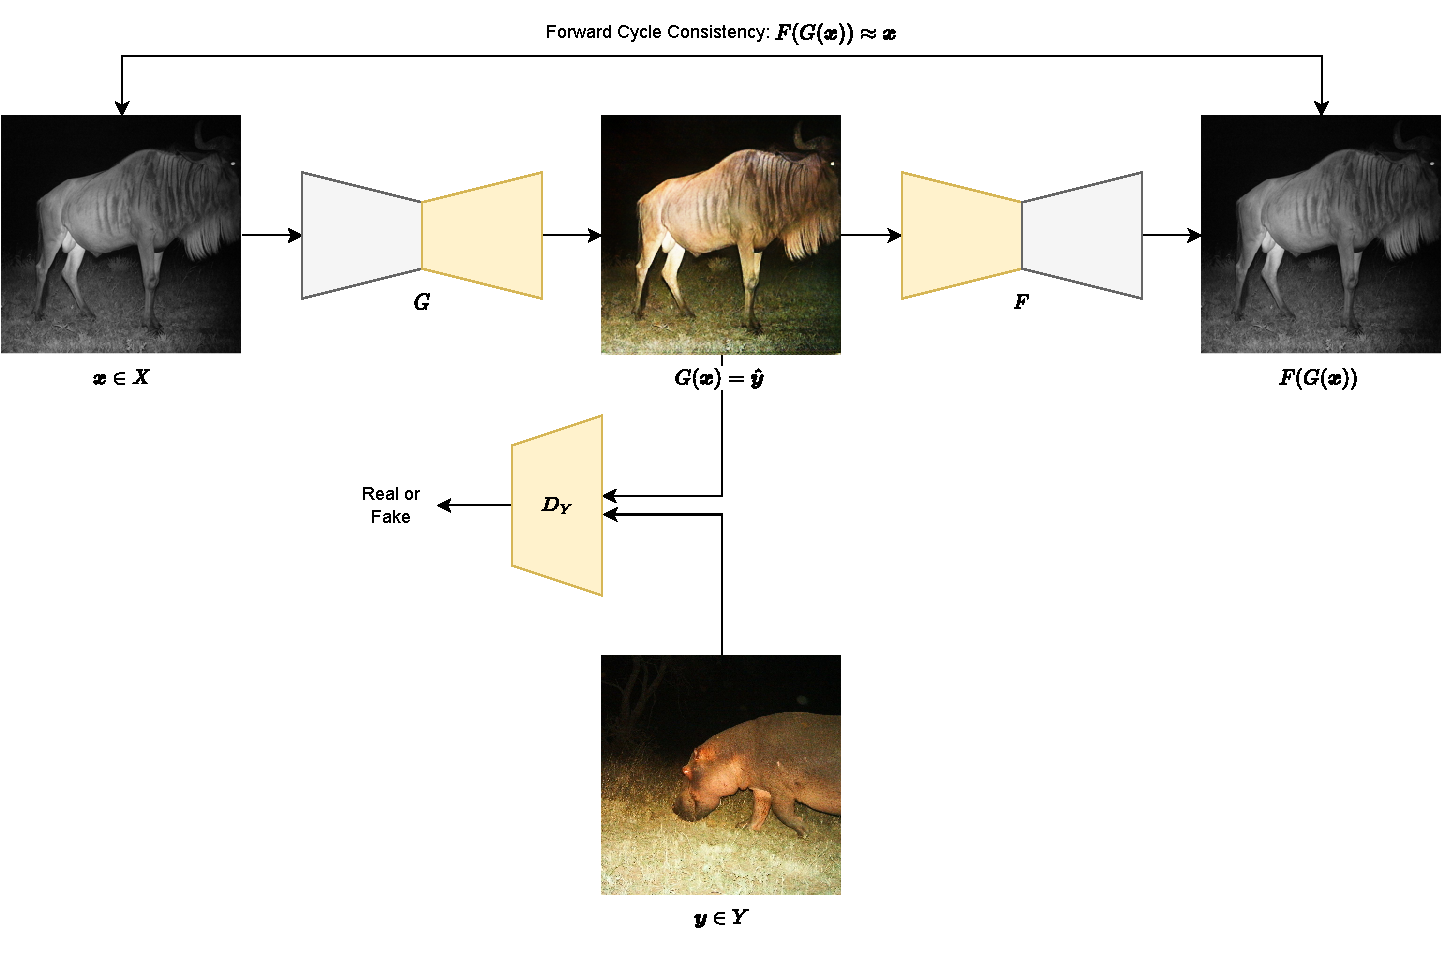
\includegraphics[width=\textwidth]{gfx/CycleGAN.pdf}
   \caption{
      \textbf{CycleGAN Schema.} Two generators $G$ and $F$ translate between both domains. Forward Cycle Consistency is ensured using the input and recovered NIR image.
      The discriminator $D_Y$ encourages the generator $G$ to learn the features of domain $\mathcal{Y}$ \parencite{cyclegan_orig,mehri2019colorizing}.
   }
   \label{fig:cycle-gan}
\end{figure}

\subsubsection*{Cycle Consistency Loss}
This objective is written as a loss function $\mathcal{L}_{cyc}(G, F)$ which uses an L1 norm to encourage cycle consistency (\autoref{eqn:cyc}).
In addition to \textit{forward cycle consistency}, CycleGAN also utilizes \textit{backward cycle consistency} which means that for $\y \in \mathcal{Y}$, $G(F(\y)) \approx \y$ \parencite{cyclegan_orig} applies, too (\autoref{fig:cycle-gan}).

\begin{equation}
   \label{eqn:cyc}
   \begin{aligned}
      \mathcal{L}_{cyc}(G, F) = \underbrace{\mathbb{E}_{\x \sim X}\left[||F(G(\x)) - \x||_1\right]}_{\text{forward cycle consistency}} +
      \underbrace{\mathbb{E}_{\y \sim Y}\left[||G(F(\y))) - \y||_1\right]}_{\textit{backward cycle consistency}}
   \end{aligned}
\end{equation}

In addition to the L1 cycle consistency loss, \citeauthor*{mehri2019colorizing} propose using \textit{structural similarity index measurement} (SSIM) as the second cycle consistency loss \parencite{mehri2019colorizing}.
Contrary to the L1 loss, SSIM measures the differences between the images not by the absolute image intensity values but by comparing two images based on luminance-, contrast- and structural similarity \parencite{ssim}.

Using measurements for luminance $l(\y_1, \y_2)$, contrast $c(\y_1,\y_2)$ and structure comparison $s(\y_1, \y_2)$, we can obtain the overall structural similarity
index $SSIM(\y_1, \y_2)$ as multiplication of each component (\autoref{eqn:ssim}) \parencite{ssim}.

\begin{equation}
   \label{eqn:ssim}
   \begin{aligned}
      SSIM(\y_1, \y_2) = l(\y_1, \y_2) \cdot c(\y_1,\y_2) \cdot s(\y_1, \y_2)
   \end{aligned}
\end{equation}

The SSIM is obtained using a moving Gaussian window on the image, and therefore the SSIM \textbf{difference} between two images $\overline{SSIM(\y_1,\y_2)}$ is calculated as follows (\autoref{eqn:ssim_difference}).
Let $\y_{1,j}$ and $\y_{2,j}$ be the image contents of the $j$-th local patch using the Gaussian window, where $M$ is the number of Gaussian windows.

\begin{equation}
   \label{eqn:ssim_difference}
   \begin{aligned}
      \overline{SSIM(\y_1,\y_2)} = \frac{1}{M}\sum_{j=1}^{M}1 - SSIM(\y_{1,j},\y_{2,j})
   \end{aligned}
\end{equation}

Finally, the loss of cycle consistency $\mathcal{L}_{SSIM}(G, F)$ can be constructed using the differences in the SSIMs between the images (\autoref{eqn:ssim_loss}).

\begin{equation}
   \label{eqn:ssim_loss}
   \begin{aligned}
      \mathcal{L}_{SSIM}(G,F) & = \mathbb{E}_{\x \sim X}\left[\overline{SSIM(F(G(\x)), \x)}\right] + \mathbb{E}_{\y \sim Y}\left[\overline{SSIM(G(F(\y)), \y)}\right]
   \end{aligned}
\end{equation}


\subsubsection*{Relativistic Adversarial Loss}
For both generators, adversarial discriminators $D_X$ and $D_Y$ are introduced where $D_X$ has the aim of distinguishing between real images
$X$ and generated images $\{F(\y)\}$ and $D_Y$ for $Y$ and $\{G(\x)\}$.
For both, we apply a relativistic GAN, in particular, \textit{RaLSGAN} \parencite{mehri2019colorizing,rel_gan}.
\autoref{eqn:ralsgan} demonstrates the RaLSGAN loss for the generator $G$ ($\mathcal{L}^G_{RaLSGAN}(G,D_Y,X,Y)$) and its discriminator
$D_Y$ ($\mathcal{L}^D_{RaLSGAN}(G,D_Y,X,Y)$) (\autoref{fig:cycle-gan}). The loss for $F$ and $D_X$ is defined in the same way as for $G$ and $D_Y$ \parencite{rel_gan}.

\begin{equation}
   \label{eqn:ralsgan}
   \begin{aligned}
      \mathcal{L}^{D_Y}_{RaLSGAN}(G,D_Y,X,Y) & = \mathbb{E}_{\y \sim Y}\left[(D_Y(\y) - \mathbb{E}_{\x \sim X} D_Y(G(\x)) - 1)^2 \right] \\
                                             & + \mathbb{E}_{\x \sim X}\left[(D_Y(G(\x)) - \mathbb{E}_{\y \sim Y} D_Y(\y) + 1)^2 \right] \\
      \mathcal{L}^G_{RaLSGAN}(G,D_Y,X,Y)     & = \mathbb{E}_{\x \sim X}\left[(D_Y(G(\x)) - \mathbb{E}_{\y \sim Y} D_Y(\y) - 1)^2 \right] \\
                                             & + \mathbb{E}_{\y \sim Y}\left[(D_Y(\y) - \mathbb{E}_{\x \sim X} D_Y(G(\x)) + 1)^2 \right]
   \end{aligned}
\end{equation}

\subsection*{Identity Loss}
Lastly, the identity loss has the aim of regulating the generator:
If an image already appears like a colored RGB image, it should not be modified.
This leads to the identity loss $\mathcal{L}_{identiy}$ (\autoref{eqn:identity_loss}) \parencite{mehri2019colorizing}.

\begin{equation}
   \label{eqn:identity_loss}
   \begin{aligned}
      \mathcal{L}_{identiy}(G, F) = \mathbb{E}_{\x \sim X} \left[||G(\x) - \x||_1\right] + \mathbb{E}_{\y \sim Y} \left[||G(\y) - \y||_1\right]
   \end{aligned}
\end{equation}

\subsection*{Full Objective}
All those four loss functions lead to an additive final loss function (\autoref{eqn:cycle_gan_total_loss}) \parencite{mehri2019colorizing}.
$\lambda$ and $\gamma$ are weights for the relative importance of the L1 cycle consistency loss and the identity loss.

\begin{equation}
   \label{eqn:cycle_gan_total_loss}
   \begin{aligned}
      \mathcal{L} = \lambda \mathcal{L}_{cyc} + \mathcal{L}_{SSIM} + \gamma \mathcal{L}_{identity}(G,F) + \mathcal{L}_{RaLSGAN}^G(G,D_Y,X,Y) + \mathcal{L}_{RaLSGAN}^F(F,D_X,Y,X)
   \end{aligned}
\end{equation}

\subsubsection*{U-Net}
In praxis, both functions $G$ and $F$ are generation networks. Contrary to the ResNet generators \parencite{resnet} \citeauthor{cyclegan_orig} used in the original CycleGAN \parencite{cyclegan_orig},
\citeauthor*{mehri2019colorizing} propose U-Net generators \parencite{unet}, because they perform better in learning the color \parencite{mehri2019colorizing}.
Additionally, U-Net generators also need less computational time for training compared to ResNet \parencite{mehri2019colorizing}.
We input all three (equal) channels of the NIR image into the generator and receive an RGB image as output.
All activations of the encode-blocks (except the last one) are inputs for two blocks:
The following encode- as well as the corresponding decode-block. This is called a skip connection \parencite{unet} (\autoref{fig:unet}). All decode-blocks (except the first one) receive input from the previous decode-block, as well as the corresponding encode-block.
This leads to an architecture that can learn to "choose" how deep the feature abstraction should be \parencite{unet}.

\begin{figure}[h]
   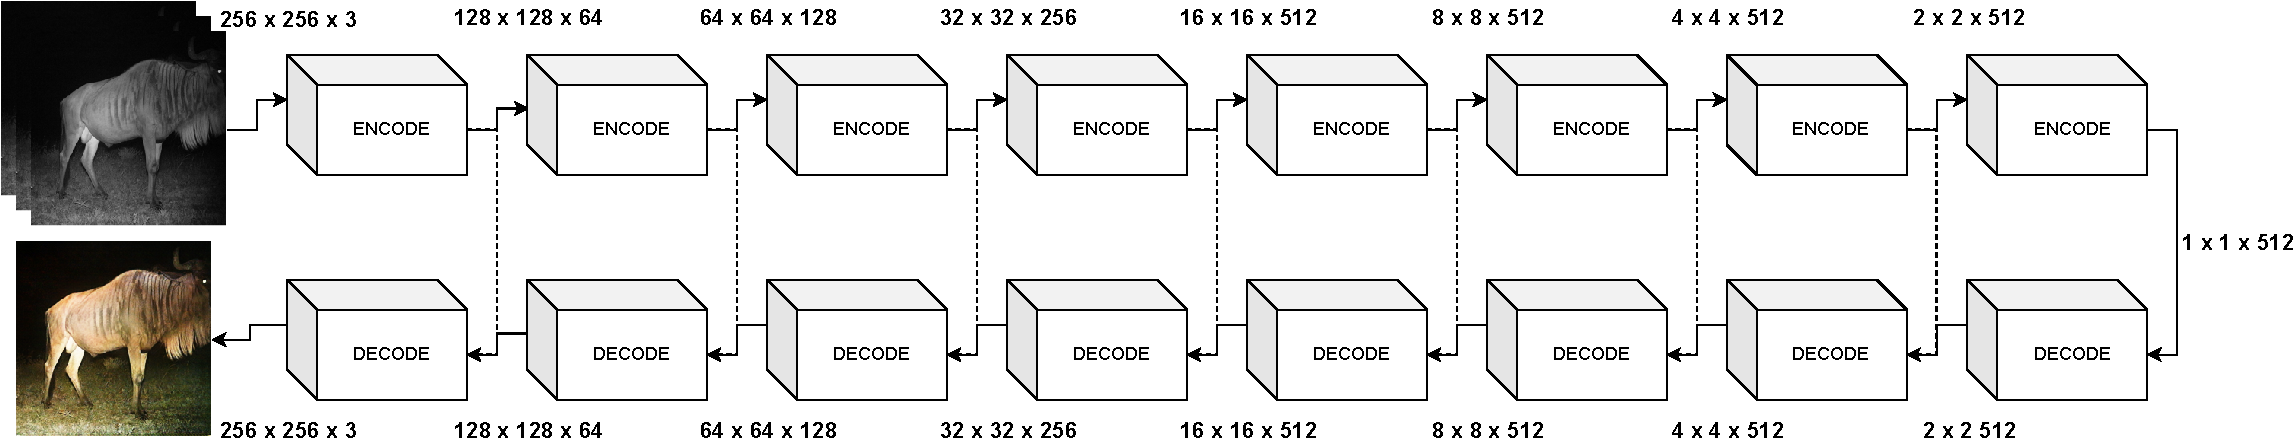
\includegraphics[width=\textwidth]{gfx/CycleGAN-Unet.pdf}
   \caption{
      U-Net generator $G$ used in CycleGAN \parencite{unet,mehri2019colorizing}
   }
   \label{fig:unet}
\end{figure}

\subsubsection*{Optimizations}
\Citeauthor*{ttur} demonstrated that using the \textit{two timescale update rule} (TTUR), which states that when the generator and the discriminator have different learning rates,
mode collapse can be prevented in image translation tasks using GANs \parencite{ttur}.
Inspired by this, \citeauthor*{mehri2019colorizing} propose utilizing two learning rates for the CycleGAN architecture \parencite{mehri2019colorizing}.

Additionally, \citeauthor*{mehri2019colorizing} propose the use of \textit{spectral normalization}, a technique introduced by \Citeauthor*{spectral_norm}, to stabilize the training of the discriminators $D_X$ and $D_Y$ \parencite{spectral_norm, mehri2019colorizing}.

Finally, \citeauthor*{mehri2019colorizing} observe that while the cycle consistency loss helps in the early training stages, it hinders the network in the later stages in generating realistic images \parencite{mehri2019colorizing}.
Therefore, \citeauthor*{mehri2019colorizing} propose to decrease the weight of the cycle consistency loss after half of the training process \parencite{mehri2019colorizing}.

\section{Diffusion Models}
\subsection{Prerequisites}
\subsection{Loss-Based Conditional Sampling}
\subsection{Strong-Guided Conditional Sampling}

\chapter{Evaluation and Discussion}
\label{chap:evaluation-and-discussion}

\section{Evaluation Metrics}

As NIR colorization has two main application contexts: providing human users more interpretable images and to improve object recognition results by enriching the input with more information.
To assess the effectiveness of both models, we define qualitative evaluation categories and quantitative evaluation metrics based on their ability to achieve these goals.

\subsection{Quantitative Evaluation Metrics}
Due to the unpaired setting, in the quantitative evaluation classic solutions, such as the difference between the absolute intensity values or SSIM \parencite{ssim}, cannot be applied. Fortunately, methods for comparing the general image similarity of two sets, such as FID \parencite{ttur} or
comparing classification results using an off-the-shelf network, are well known to quantitatively assess the quality of image translation.

\subsubsection*{FID}
To measure how close the generated images are to the real images concerning human perception, the \textit{Fréchet Inception Distance} (FID) \parencite{ttur} is a commonly used metric.
It empirically estimates how the human eye perceives images for a set of images and computes the distance between two such set representations.
First, a pre-trained InceptionV3 model evaluates each image of the image set and the activation of the last layer is considered the "human perception approximation".
Then for all activation vectors of the evaluated images in the images set, a multidimensional Gaussian is fitted over those activation vectors.
This is done for two image sets, and later the two Gaussians are compared using the Fréchet distance \parencite{ttur}.
Intuitively, if the generated images are realistic, the statistics of features in a classification network should be similar to the real ones.

\todo{Add figure visualizing FID}

\label{sec:evaluate-fid}
\todo{Discuss usage of FID}

\subsection{Qualitative Evaluation Methods}
For qualitative evaluation, we define categories on how we determine the superior generated images. These are again based on the two main application contexts.

The first category describes the \textit{naturality} of an image, where the generated images should resemble how humans perceive the world, without artifacts or periodic patterns that can affect visual perception.

The second category refers to the \textit{content preservation} of the input image. This should help humans as well as object detection systems to find and classify animals accurately.

\textit{Hallucinations}, as artifacts or scene elements that are not in the input image, contradict naturality and content preservation, and therefore are undesirable.

\section{Unconditional Diffusion Model}
First we evaluate the unconditional sampling of the diffusion model and therefore validate \parencite{diffusion-beats-gans}'s results for image synthesis in still hold for this dataset:

\begin{table}[htp!]
    \centering
    \begin{tabular}{c | c}
        Model                   & FID  $\downarrow$ \\
        \hline\hline
        CycleGAN                & 98.10             \\
        Unconditional Diffusion & 95.73
    \end{tabular}
    \caption{
        \textbf{Quantitative Evaluation.} CycleGAN and the diffusion model trained on Snapshot Serengeti \parencite{serengeti} containing only night NIR and RGB images.
        Comparing the FID calculated between the test dataset and the generated images.
    }
    \label{fig:quantitative-evaluation-unconditional-sampling}
\end{table}

\begin{figure}[htp!]
    \centering
    \todo{Better choice of images}
    \setkeys{Gin}{width=1\linewidth}
    \begin{tabularx}{\textwidth}{>{\centering\arraybackslash}X >{\centering\arraybackslash}X >{\centering\arraybackslash}X >{\centering\arraybackslash}X >{\centering\arraybackslash}X >{\centering\arraybackslash}X}
        RGB                                                                                    & CycleGAN                                                                                         & Diffusion                                                                                    & RGB                                                                                    & CycleGAN                                                                                         & Diffusion                                                                                    \\
        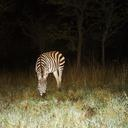
\includegraphics{gfx/unconditional-diffusion-sampling-qual/rgb_S2_B04_R3_IMAG0432.jpg} & \includegraphics{gfx/unconditional-diffusion-sampling-qual/cyclegan_S2_B06_R1_PICT0128_fake.png} & 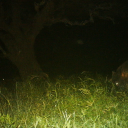
\includegraphics{gfx/unconditional-diffusion-sampling-qual/diffusion_S2_B06_R1_PICT0128.png} & 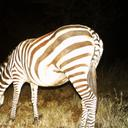
\includegraphics{gfx/unconditional-diffusion-sampling-qual/rgb_S2_B04_R3_IMAG0471.jpg} & 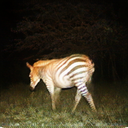
\includegraphics{gfx/unconditional-diffusion-sampling-qual/cyclegan_S2_B06_R1_PICT0279_fake.png} & 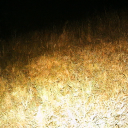
\includegraphics{gfx/unconditional-diffusion-sampling-qual/diffusion_S2_B06_R1_PICT0279.png} \\
        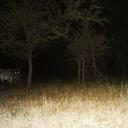
\includegraphics{gfx/unconditional-diffusion-sampling-qual/rgb_S2_B05_R1_IMAG0084.jpg} & \includegraphics{gfx/unconditional-diffusion-sampling-qual/cyclegan_S2_B06_R1_PICT0387_fake.png} & 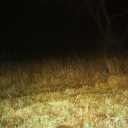
\includegraphics{gfx/unconditional-diffusion-sampling-qual/diffusion_S2_B06_R1_PICT0387.png} & 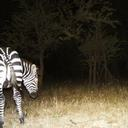
\includegraphics{gfx/unconditional-diffusion-sampling-qual/rgb_S2_B05_R1_IMAG0132.jpg} & \includegraphics{gfx/unconditional-diffusion-sampling-qual/cyclegan_S2_B06_R3_PICT1364_fake.png} & 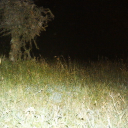
\includegraphics{gfx/unconditional-diffusion-sampling-qual/diffusion_S2_B06_R3_PICT1364.png} \\
        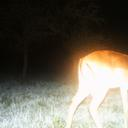
\includegraphics{gfx/unconditional-diffusion-sampling-qual/rgb_S2_B05_R2_IMAG0016.jpg} & 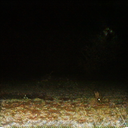
\includegraphics{gfx/unconditional-diffusion-sampling-qual/cyclegan_S2_B06_R3_PICT3848_fake.png} & 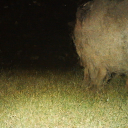
\includegraphics{gfx/unconditional-diffusion-sampling-qual/diffusion_S2_B06_R3_PICT3848.png} & 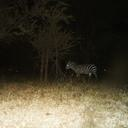
\includegraphics{gfx/unconditional-diffusion-sampling-qual/rgb_S2_B05_R3_IMAG1018.jpg} & 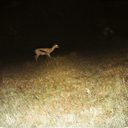
\includegraphics{gfx/unconditional-diffusion-sampling-qual/cyclegan_S2_B07_R1_PICT3274_fake.png} & 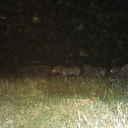
\includegraphics{gfx/unconditional-diffusion-sampling-qual/diffusion_S2_B07_R1_PICT3274.png}
    \end{tabularx}
    \caption{
        \textbf{Qualitative Evaluation.} Left to right: Sample image from the RGB domain of the Serengeti test dataset \parencite{serengeti},
        sample produced by CycleGAN \parencite{mehri} and an unconditional sample produced by the diffusion model \parencite{diffusion-beats-gans}.
    }
    \label{fig:qualitative-evaluation-unconditional-sampling}
\end{figure}

Qualitatively we observe in \autoref{fig:qualitative-evaluation-unconditional-sampling} that the diffusion model is capable to create realistic images.
As in the training dataset, many images without animal present are produced.
Images containing animals illustrates the model performs exceptionally well in creating realistic ones with matching lighting.
Only in few cases, trees are generated with undistinguishable branches. This is the only flaw which can be observed.

Quantitatively in \autoref{fig:quantitative-evaluation-unconditional-sampling} we see, the diffusion network only slightly outperforms CycleGAN's performance.
We expect clearer distinction to CycleGAN when a larger U-Net would be used, more training iterations and a larger dataset would be used. 
Compared to \textcite{diffusion-beats-gans} we had to do trade-offs due to a lack of ultra-high performant computational resources.
Nevertheless, it can be argued that this unconditional diffusion model is capable enough to be a basis for a good colorization.

\todo{Provide hyperparameter}

\section{Loss-Guided and Correction-Guided Sampling}
As introduced in \autoref{sec:conditional-sampling} we suggest a differentiation into 
\textit{loss-guided} (\autoref{sec:energy-guided-sampling}) and \textit{correction-guided} (\autoref{sec:correction-guided-sampling}) sampling.

At first sight we observe greater simplicity in defining a loss or energy rather than correcting an image.
Generally when using the correction-guided approach, the current sampled image has to be decomposed into multiple parts,
one part being the one to be modified and the second one being the remainder.
As the decomposition function must be invertible to create a functional framework, not all problems or properties are suited to be modelled like this.
Formulation as an energy is often easier to obtain and sometimes the only possibility.

In the case of near-infrared colorization both methods are implementable.
We evaluate for the context of near-infrared colorization which method should be used.
For both cases we condition using near-infrared images by assuming the intensity of the sample should be equal to the near-infrared image.
We discuss this particular conditioning method separately in \autoref{sec:nir-as-intensity-approximation-evaluation}.
In \autoref{fig:qualitative-evaluation-loss-guided-vs-correction-guided} we demonstrate the difference when formulating exactly the same property as energy-guided sampling and as correction-guided sampling.
It can be observed that the contours appear generally more noisy in the loss-guided sampling.
This observation is also quantitatively reflected, the FID of the loss-guided sampling is $23.64$ points higher than of the correction-guided approach (\autoref{fig:quantitative-evaluation-loss-guided-vs-correction-guided}).

\begin{figure}[htp!]
    \centering
    \setkeys{Gin}{width=1\linewidth}
    \begin{tabularx}{\textwidth}{>{\centering\arraybackslash}X >{\centering\arraybackslash}X >{\centering\arraybackslash}X >{\centering\arraybackslash}X >{\centering\arraybackslash}X >{\centering\arraybackslash}X}
        \centering NIR                                                                                            & Correction-Guided                                                                                                                 & Loss-Guided                                                                                                                 & NIR                                                                                                       & Correction-Guided                                                                                                                 & Loss-Guided                                                                                                                 \\
        \includegraphics{gfx/diffusion-sampling-loss-guided-vs-correction-guided-qual/nir_S2_B06_R1_PICT0128.jpg} & 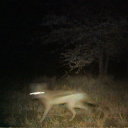
\includegraphics{gfx/diffusion-sampling-loss-guided-vs-correction-guided-qual/diffusion-correction-guided_S2_B06_R1_PICT0128.png} & 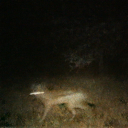
\includegraphics{gfx/diffusion-sampling-loss-guided-vs-correction-guided-qual/diffusion-loss-guided_S2_B06_R1_PICT0128.png} & \includegraphics{gfx/diffusion-sampling-loss-guided-vs-correction-guided-qual/nir_S2_B06_R1_PICT0279.jpg} & 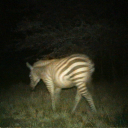
\includegraphics{gfx/diffusion-sampling-loss-guided-vs-correction-guided-qual/diffusion-correction-guided_S2_B06_R1_PICT0279.png} & 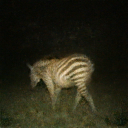
\includegraphics{gfx/diffusion-sampling-loss-guided-vs-correction-guided-qual/diffusion-loss-guided_S2_B06_R1_PICT0279.png} \\
        \includegraphics{gfx/diffusion-sampling-loss-guided-vs-correction-guided-qual/nir_S2_B06_R1_PICT0387.jpg} & 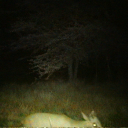
\includegraphics{gfx/diffusion-sampling-loss-guided-vs-correction-guided-qual/diffusion-correction-guided_S2_B06_R1_PICT0387.png} & 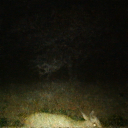
\includegraphics{gfx/diffusion-sampling-loss-guided-vs-correction-guided-qual/diffusion-loss-guided_S2_B06_R1_PICT0387.png} & \includegraphics{gfx/diffusion-sampling-loss-guided-vs-correction-guided-qual/nir_S2_B06_R3_PICT1364.jpg} & 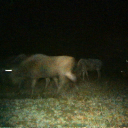
\includegraphics{gfx/diffusion-sampling-loss-guided-vs-correction-guided-qual/diffusion-correction-guided_S2_B06_R3_PICT1364.png} & 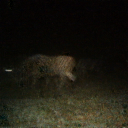
\includegraphics{gfx/diffusion-sampling-loss-guided-vs-correction-guided-qual/diffusion-loss-guided_S2_B06_R3_PICT1364.png} \\
        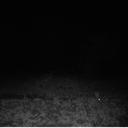
\includegraphics{gfx/diffusion-sampling-loss-guided-vs-correction-guided-qual/nir_S2_B06_R3_PICT3848.jpg} & 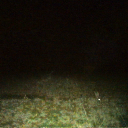
\includegraphics{gfx/diffusion-sampling-loss-guided-vs-correction-guided-qual/diffusion-correction-guided_S2_B06_R3_PICT3848.png} & 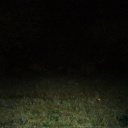
\includegraphics{gfx/diffusion-sampling-loss-guided-vs-correction-guided-qual/diffusion-loss-guided_S2_B06_R3_PICT3848.png} & 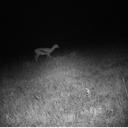
\includegraphics{gfx/diffusion-sampling-loss-guided-vs-correction-guided-qual/nir_S2_B07_R1_PICT3274.jpg} & 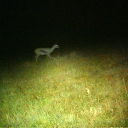
\includegraphics{gfx/diffusion-sampling-loss-guided-vs-correction-guided-qual/diffusion-correction-guided_S2_B07_R1_PICT3274.png} & 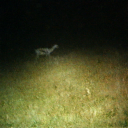
\includegraphics{gfx/diffusion-sampling-loss-guided-vs-correction-guided-qual/diffusion-loss-guided_S2_B07_R1_PICT3274.png}
    \end{tabularx}
    \caption{
        \todo{Add Caption}
    }
    \label{fig:qualitative-evaluation-loss-guided-vs-correction-guided}
\end{figure}

\begin{table}[htp!]
    \centering
    \begin{tabular}{c | c}
        Model             & FID  $\downarrow$ \\
        \hline\hline
        Correction-Guided & 105.00            \\
        Loss-Guided       & 128.64
    \end{tabular}
    \caption{
        \todo{Add Caption}
    }
    \label{fig:quantitative-evaluation-loss-guided-vs-correction-guided}
\end{table}

\todo{Provide intuition for this observation !}

\todo{Unify with observations of \autoref{sec:high-pass-filter-evaluation}}

\section{Conditioning the Near-Infrared}
\subsection{NIR as Intensity Approximation}
\label{sec:nir-as-intensity-approximation-evaluation}
\Textcite{sbgm} already suggested colorization methods using diffusion models.
Although in comparison visible light, near-infrared light has different reflection properties,
we could ignore this property and assume the NIR intensity to be a good approximation of the visual light's intensity.
Therefore, we start by implementing colorization as \autoref{sec:correction-guided-sampling-gray-scale-colorization} and evaluate 
this idea empirically.

\begin{figure}[htp!]
    \centering
    \setkeys{Gin}{width=1\linewidth}
    \begin{tabularx}{\textwidth}{>{\centering\arraybackslash}X >{\centering\arraybackslash}X >{\centering\arraybackslash}X >{\centering\arraybackslash}X >{\centering\arraybackslash}X >{\centering\arraybackslash}X}
        NIR                                                                                & CycleGAN                                                                                     & Diffusion                                                                                & NIR                                                                                & CycleGAN                                                                                     & Diffusion                                                                                \\
        \includegraphics{gfx/diffusion-sampling-intensity-qual/nir_S2_B06_R1_PICT0128.jpg} & \includegraphics{gfx/diffusion-sampling-intensity-qual/cyclegan_S2_B06_R1_PICT0128_fake.png} & 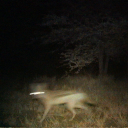
\includegraphics{gfx/diffusion-sampling-intensity-qual/diffusion_S2_B06_R1_PICT0128.png} & \includegraphics{gfx/diffusion-sampling-intensity-qual/nir_S2_B06_R1_PICT0279.jpg} & 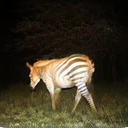
\includegraphics{gfx/diffusion-sampling-intensity-qual/cyclegan_S2_B06_R1_PICT0279_fake.png} & 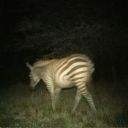
\includegraphics{gfx/diffusion-sampling-intensity-qual/diffusion_S2_B06_R1_PICT0279.png} \\
        \includegraphics{gfx/diffusion-sampling-intensity-qual/nir_S2_B06_R1_PICT0387.jpg} & \includegraphics{gfx/diffusion-sampling-intensity-qual/cyclegan_S2_B06_R1_PICT0387_fake.png} & 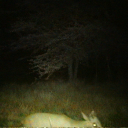
\includegraphics{gfx/diffusion-sampling-intensity-qual/diffusion_S2_B06_R1_PICT0387.png} & \includegraphics{gfx/diffusion-sampling-intensity-qual/nir_S2_B06_R3_PICT1364.jpg} & \includegraphics{gfx/diffusion-sampling-intensity-qual/cyclegan_S2_B06_R3_PICT1364_fake.png} & 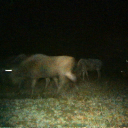
\includegraphics{gfx/diffusion-sampling-intensity-qual/diffusion_S2_B06_R3_PICT1364.png} \\
        \includegraphics{gfx/diffusion-sampling-intensity-qual/nir_S2_B06_R3_PICT3848.jpg} & \includegraphics{gfx/diffusion-sampling-intensity-qual/cyclegan_S2_B06_R3_PICT3848_fake.png} & \includegraphics{gfx/diffusion-sampling-intensity-qual/diffusion_S2_B06_R3_PICT3848.png} & \includegraphics{gfx/diffusion-sampling-intensity-qual/nir_S2_B07_R1_PICT3274.jpg} & \includegraphics{gfx/diffusion-sampling-intensity-qual/cyclegan_S2_B07_R1_PICT3274_fake.png} & \includegraphics{gfx/diffusion-sampling-intensity-qual/diffusion_S2_B07_R1_PICT3274.png}
    \end{tabularx}
    \caption{
        \textbf{Qualitative Evaluation.} Left to right: Image from the NIR domain of the Serengeti test dataset \parencite{serengeti},
        corresponding image generated by CycleGAN \parencite{mehri} and corresponding sample generated by our diffusion model approach.
    }
    \label{fig:qualitative-evaluation-intensity}
\end{figure}

In \autoref{fig:qualitative-evaluation-intensity} we show evaluation results of this approach. 
Qualitatively we can observe those generated images are faithful to the input image (\autoref{fig:qualitative-evaluation-intensity}).
It is to be mentioned that faithfulness to the input image is not a quality learned by the network, but a design choice of the sampling procedure.
Most noteworthy is that the colors estimated by the diffusion model appear realistic.
Qualitative weaknesses in the colorization can be observed when analyzing the zebra image:
While CycleGAN colorizes the main zebra body as black and white, the diffusion network produces an orange-black zebra.
This can be traced back to a conceptional weakness.
The diffusion network is forced to reuse the intensity of the NIR image.
The zebra in the NIR image is gray-black and therefore the network is not capable in generating high intensity pixels.
CycleGAN on the other-hand is not restricted by design to change the intensity.
It is merely trained to produce invertible images.

\begin{table}[htp!]
    \centering
    \begin{tabular}{c | c}
        Model                                           & FID  $\downarrow$ \\
        \hline\hline
        CycleGAN                                        & 98.10             \\
        Unconditional Diffusion                         & 96.03             \\
        \textbf{Conditional Diffusion} \parencite{sbgm} & \textbf{105.00}
    \end{tabular}
    \caption{
        \textbf{Quantitative Evaluation.} CycleGAN and the diffusion model trained on Snapshot Serengeti \parencite{serengeti} containing only night NIR and RGB images.
        Comparing the FID calculated between the test dataset and the generated images.
    }
    \label{fig:qualitative-evaluation-full-high-pass}
\end{table}


Similar to the minor qualitative weakness, we also observe the FID of this naive approach to be $6.9$ FID points worse than CycleGAN.
Additionally, we see a gap between the sampling the unconditional diffusion model produces our method according to \Citeauthor*{sbgm} of $8.97$ FID points \parencite{sbgm}.
This indicates that this method is too restrictive to allow competitive image generation.


\todo{Explanation why approximation even works, night, few vegetation, ...}

To improve the intuition of the difference between the intensities, we consider CycleGAN's intensities a good approximation of the real visible intensity.
We compare this with the near-infrared intensity in \autoref{fig:heatmap-cycle-gan-intensity}.

\begin{figure}[htp!]
    \centering
    \includegraphics[width=\textwidth]{gfx/heatmap-nir-cycle-gan-intensity-diff.png}
    \caption{
        \todo{Better integration (using pdf or so); Best: Direct latex code}
        Absolute difference between CycleGAN's intensity and the NIR image.
        Left to Right: Intensity calculated by images generated by CycleGAN, Near-Infared image \parencite{serengeti} and difference between both.
    }
    \label{fig:heatmap-cycle-gan-intensity}
\end{figure}

We first observe the pattern, that CycleGAN does especially enlighten the foreground and with that the lower regions of the image.
The same holds for animals in the foreground such as the fox or zebra.
Indeed, while comparing the intensity of near-infrared and the incandescent image in the Serengeti dataset \parencite{serengeti}
this pattern is observable again:
Generally the light in incandescent images appears to be stronger and therefore foreground objects are more illuminated.

Naturally when fixing the intensity of the NIR image for the diffusion sampling, such distinct features of the incandescent images is not achievable,
and therefore a higher FID is not unexpected.

As it is now clear that this physical inaccuracy we accepted, might influence the performance of our sampling, it is not yet clear to what extent.
To investigate this, in \autoref{fig:qualitative-evaluation-cyclegan-conditional-sampling} choose to use the same sampling method as before, but instead use the intensities produced by CycleGAN as input to the diffusion sampling.

\begin{figure}[htp!]
    \centering
    \setkeys{Gin}{width=1\linewidth}
    \begin{tabularx}{\textwidth}{>{\centering\arraybackslash}X >{\centering\arraybackslash}X >{\centering\arraybackslash}X >{\centering\arraybackslash}X >{\centering\arraybackslash}X >{\centering\arraybackslash}X}
        NIR                                                                              & CycleGAN                                                                                   & Diffusion with CycleGAN Input                                                                    & NIR                                                                              & CycleGAN                                                                                   & Diffusion with CycleGAN Input                                                                    \\
        \includegraphics{gfx/conditional-with-cycle-gan-qual/nir_S2_B06_R1_PICT0128.jpg} & \includegraphics{gfx/conditional-with-cycle-gan-qual/cyclegan_S2_B06_R1_PICT0128_fake.png} & \includegraphics{gfx/conditional-with-cycle-gan-qual/diff_cycle_gan_S2_B06_R1_PICT0128_fake.png} & \includegraphics{gfx/conditional-with-cycle-gan-qual/nir_S2_B06_R1_PICT0279.jpg} & \includegraphics{gfx/conditional-with-cycle-gan-qual/cyclegan_S2_B06_R1_PICT0279_fake.png} & \includegraphics{gfx/conditional-with-cycle-gan-qual/diff_cycle_gan_S2_B06_R1_PICT0279_fake.png} \\
        \includegraphics{gfx/conditional-with-cycle-gan-qual/nir_S2_B06_R1_PICT0387.jpg} & \includegraphics{gfx/conditional-with-cycle-gan-qual/cyclegan_S2_B06_R1_PICT0387_fake.png} & \includegraphics{gfx/conditional-with-cycle-gan-qual/diff_cycle_gan_S2_B06_R1_PICT0387_fake.png} & \includegraphics{gfx/conditional-with-cycle-gan-qual/nir_S2_B06_R3_PICT1364.jpg} & \includegraphics{gfx/conditional-with-cycle-gan-qual/cyclegan_S2_B06_R3_PICT1364_fake.png} & \includegraphics{gfx/conditional-with-cycle-gan-qual/diff_cycle_gan_S2_B06_R3_PICT1364_fake.png} \\
        \includegraphics{gfx/conditional-with-cycle-gan-qual/nir_S2_B06_R3_PICT3848.jpg} & \includegraphics{gfx/conditional-with-cycle-gan-qual/cyclegan_S2_B06_R3_PICT3848_fake.png} & \includegraphics{gfx/conditional-with-cycle-gan-qual/diff_cycle_gan_S2_B06_R3_PICT3848_fake.png} & \includegraphics{gfx/conditional-with-cycle-gan-qual/nir_S2_B07_R1_PICT3274.jpg} & \includegraphics{gfx/conditional-with-cycle-gan-qual/cyclegan_S2_B07_R1_PICT3274_fake.png} & \includegraphics{gfx/conditional-with-cycle-gan-qual/diff_cycle_gan_S2_B07_R1_PICT3274_fake.png}
    \end{tabularx}
    \caption{
        \todo{Add caption}
    }
    \label{fig:qualitative-evaluation-cyclegan-conditional-sampling}
\end{figure}

\begin{table}[htp!]
    \centering
    \begin{tabular}{c | c}
        Model                                    & FID  $\downarrow$ \\
        \hline\hline
        CycleGAN                                 & 98.10             \\
        Diffusion with CycleGAN Intensity Inputs & \textbf{97.21}    \\
        Diffusion with NIR Inputs                & 104.04
    \end{tabular}
    \caption{
        \todo{Add caption}
    }
    \label{fig:quantitative-evaluation-cyclegan-conditional-sampling}
\end{table}


In \autoref{fig:qualitative-evaluation-cyclegan-conditional-sampling} we see that not only is the diffusion model more than capable in colorizing these pictures,
it also exceeds CycleGAN's color choices. While the zebra of CycleGAN has an orange outline at the head where it should not, the diffusion model does not make this mistake
which results in overall more realistic images.

This subtle difference between the CycleGAN and the diffusion model samples with CycleGAN intensity inputs is also visible while comparing the images quantitatively in \autoref{fig:quantitative-evaluation-cyclegan-conditional-sampling}.
The diffusion model performs better than CycleGAN when the intensities are appropriate.
Diffusion models theoretically perform best in the unconditional sampling in comparison when they being guided by unseen data.
In the unconditional setting it only performs $1.2$ FID points better (\autoref{fig:quantitative-evaluation-unconditional-sampling}). 
Therefore, we have shown that the assumption that the near-infrared intensities approximate the visual intensities well,
is the main factor explaining the difference between the quantitative results.

\subsection{High-Pass Filtering of NIR}
\label{sec:high-pass-filter-evaluation}

To improve this weakness, we can get inspired by simple NIR-RGB enhancement methods based on filters \parencite{rgb-nir-image-enhancement}.
A better approximation is to use only the high-frequencies of the near-infrared image while the low frequencies can still be sampled by the diffusion model (\autoref{sec:correction-guided-sampling-nir-colorization}).
This intuitively also gives the diffusion model freedom to sample different illumination than given by the near-infrared image.

In \autoref{fig:qualitative-evaluation-full-high-pass} we evaluate the results of this concept.

\begin{figure}[htp!]
    \centering
    \setkeys{Gin}{width=1\linewidth}
    \begin{tabularx}{\textwidth}{>{\centering\arraybackslash}X >{\centering\arraybackslash}X >{\centering\arraybackslash}X >{\centering\arraybackslash}X >{\centering\arraybackslash}X >{\centering\arraybackslash}X}
        NIR                                                                                               & Full-Pass                                                                                               & High-Pass                                                                                               & NIR                                                                                               & Full-Pass                                                                                               & High-Pass                                                                                               \\
        \includegraphics{gfx/diffusion-sampling-full-vs-high-pass-filter-qual/nir_S2_B06_R1_PICT0128.jpg} & \includegraphics{gfx/diffusion-sampling-full-vs-high-pass-filter-qual/full-pass_S2_B06_R1_PICT0128.png} & \includegraphics{gfx/diffusion-sampling-full-vs-high-pass-filter-qual/high-pass_S2_B06_R1_PICT0128.png} & \includegraphics{gfx/diffusion-sampling-full-vs-high-pass-filter-qual/nir_S2_B06_R1_PICT0279.jpg} & \includegraphics{gfx/diffusion-sampling-full-vs-high-pass-filter-qual/full-pass_S2_B06_R1_PICT0279.png} & \includegraphics{gfx/diffusion-sampling-full-vs-high-pass-filter-qual/high-pass_S2_B06_R1_PICT0279.png} \\
        \includegraphics{gfx/diffusion-sampling-full-vs-high-pass-filter-qual/nir_S2_B06_R1_PICT0387.jpg} & \includegraphics{gfx/diffusion-sampling-full-vs-high-pass-filter-qual/full-pass_S2_B06_R1_PICT0387.png} & \includegraphics{gfx/diffusion-sampling-full-vs-high-pass-filter-qual/high-pass_S2_B06_R1_PICT0387.png} & \includegraphics{gfx/diffusion-sampling-full-vs-high-pass-filter-qual/nir_S2_B06_R3_PICT1364.jpg} & \includegraphics{gfx/diffusion-sampling-full-vs-high-pass-filter-qual/full-pass_S2_B06_R3_PICT1364.png} & \includegraphics{gfx/diffusion-sampling-full-vs-high-pass-filter-qual/high-pass_S2_B06_R3_PICT1364.png} \\
        \includegraphics{gfx/diffusion-sampling-full-vs-high-pass-filter-qual/nir_S2_B06_R3_PICT3848.jpg} & \includegraphics{gfx/diffusion-sampling-full-vs-high-pass-filter-qual/full-pass_S2_B06_R3_PICT3848.png} & \includegraphics{gfx/diffusion-sampling-full-vs-high-pass-filter-qual/high-pass_S2_B06_R3_PICT3848.png} & \includegraphics{gfx/diffusion-sampling-full-vs-high-pass-filter-qual/nir_S2_B07_R1_PICT3274.jpg} & \includegraphics{gfx/diffusion-sampling-full-vs-high-pass-filter-qual/full-pass_S2_B07_R1_PICT3274.png} & \includegraphics{gfx/diffusion-sampling-full-vs-high-pass-filter-qual/high-pass_S2_B07_R1_PICT3274.png}
    \end{tabularx}
    \caption{
        \todo{Add caption}
    }
    \label{fig:qualitative-evaluation-full-high-pass}
\end{figure}

\begin{table}[htp!]
    \centering
    \begin{tabular}{c | c}
        Strategy      & FID  $\downarrow$ \\
        \hline\hline
        Full-Pass     & 105.00            \\
        High-Pass     & 95.49             \\
        Unconditional & 96.02
    \end{tabular}
    \caption{
        \todo{Add caption}
    }
    \label{fig:quantitative-evaluation-full-high-pass}
\end{table}


As expected the diffusion now using the high-pass filter can manipulate the illumination of the scene.
For example, we observe for left top image now, that not only the fox itself but also the environment has an orange-lighting as typically found in the training dataset.
This reduction in restriction also positively influences the quantitative measurements:
This method achieves a FID of $95.49$ which is even $0.53$ FID points better than the unconditional sampling (\autoref{fig:quantitative-evaluation-full-high-pass}).

\todo{Resolve conflict to statement: "unconditional sampling is always the best" }

\todo{Discuss the qualitative negative points $\rightarrow$ hallucinations}

\subsection{Influence of Hyperparameter Sigma}
\label{sec:influence-of-sigma-evaluation}

\todo{Write}

\section{Diffusion and GAN}
\label{sec:diffusion-vs-cyclegan}
To study the difference between diffusion models and generative adversarial networks for near-infrared image colorization, we compare them for two specialized problems.

First we evaluate the performances on the Caltech Camera Traps dataset (\autoref{sec:cct}) by \Citeauthor*{caltech}.
The near-infrared images in the dataset are mostly taken during the night, while the color images are from the daytime \parencite{caltech}.
Both networks are required to translate mostly night near-infrared images to colored images while having mostly seen day images.
This results in artificial difficulty for the networks (\autoref{sec:diffusion-vs-cyclegan-day}).

Secondly we evaluate both networks on a more application-oriented dataset.
The subset of the Serengeti dataset we use consists mostly of night images for the near infrared domain as for the colored domain.
As near-infared applications lie for the most part in generating high-quality night images this is closer to an application context.
Because the networks are not required to perform a translation to colored night images, without having seen many of those, we consider
this specialized problem as easier, which is also visible in the quality of the results (\autoref{sec:diffusion-vs-cyclegan-night})

\subsection{Extended Dataset --- Robustness}
\label{sec:diffusion-vs-cyclegan-day}
Using the Caltech Camera Traps data split we introduced in \autoref{sec:cct},
we train an unconditional diffusion model on the mostly colored daytime images from the training dataset.

Our unconditional model is evaluated first, to validate the model did learn to approximate the target distribution well.
As visible in \autoref{fig:qualitative-evaluation-unconditional-sampling-caltech} qualitatively the diffusion network
produces highly realistic images matching the style and diversity of the test dataset well.
Quantitatively the samples achieve a fréchet inception distance of $100.22$ to the test data set.
Compared with other FIDs in this work we consider it a good value.

\begin{figure}[htp!]
    \centering
    \setkeys{Gin}{width=1\linewidth}
    \begin{tabularx}{\textwidth}{>{\centering\arraybackslash}X >{\centering\arraybackslash}X >{\centering\arraybackslash}X >{\centering\arraybackslash}X >{\centering\arraybackslash}X >{\centering\arraybackslash}X}
        RGB                                                                                                              & Diffusion                                                                               & RGB                                                                                                              & Diffusion                                                                               & RGB                                                                                                              & Diffusion                                                                               \\
        \includegraphics{gfx/unconditional-diffusion-sampling-caltech-qual/rgb_5858c0dc-23d2-11e8-a6a3-ec086b02610b.jpg} & \includegraphics{gfx/unconditional-diffusion-sampling-caltech-qual/diffusion_00000.png} & \includegraphics{gfx/unconditional-diffusion-sampling-caltech-qual/rgb_585a640e-23d2-11e8-a6a3-ec086b02610b.jpg} & \includegraphics{gfx/unconditional-diffusion-sampling-caltech-qual/diffusion_00001.png} & \includegraphics{gfx/unconditional-diffusion-sampling-caltech-qual/rgb_585a6486-23d2-11e8-a6a3-ec086b02610b.jpg} & \includegraphics{gfx/unconditional-diffusion-sampling-caltech-qual/diffusion_00002.png} \\
        \includegraphics{gfx/unconditional-diffusion-sampling-caltech-qual/rgb_585dab96-23d2-11e8-a6a3-ec086b02610b.jpg} & \includegraphics{gfx/unconditional-diffusion-sampling-caltech-qual/diffusion_00003.png} & \includegraphics{gfx/unconditional-diffusion-sampling-caltech-qual/rgb_585f4d99-23d2-11e8-a6a3-ec086b02610b.jpg} & \includegraphics{gfx/unconditional-diffusion-sampling-caltech-qual/diffusion_00004.png} & \includegraphics{gfx/unconditional-diffusion-sampling-caltech-qual/rgb_585f4fbd-23d2-11e8-a6a3-ec086b02610b.jpg} & \includegraphics{gfx/unconditional-diffusion-sampling-caltech-qual/diffusion_00005.png} \\
        \includegraphics{gfx/unconditional-diffusion-sampling-caltech-qual/rgb_5860ef9d-23d2-11e8-a6a3-ec086b02610b.jpg} & \includegraphics{gfx/unconditional-diffusion-sampling-caltech-qual/diffusion_00006.png} & \includegraphics{gfx/unconditional-diffusion-sampling-caltech-qual/rgb_58629181-23d2-11e8-a6a3-ec086b02610b.jpg} & \includegraphics{gfx/unconditional-diffusion-sampling-caltech-qual/diffusion_00007.png} & \includegraphics{gfx/unconditional-diffusion-sampling-caltech-qual/rgb_58629415-23d2-11e8-a6a3-ec086b02610b.jpg} & \includegraphics{gfx/unconditional-diffusion-sampling-caltech-qual/diffusion_00008.png}
    \end{tabularx}
    \caption{
        \todo{Add caption}
    }
    \label{fig:qualitative-evaluation-unconditional-sampling-caltech}
\end{figure}

Next our CycleGAN network is trained with images from both domains to learn a function while maintaining a cycle-consistency property according to \autoref{sec:methods-cycle-gan}.
We sample using our sampling procedure with the diffusion model given the near-infrared images of the test dataset (\todo{}) and simultaneously
sample using CycleGAN.

\begin{figure}[htp!]
    \centering
    \setkeys{Gin}{width=1\linewidth}
    \begin{tabularx}{\textwidth}{>{\centering\arraybackslash}X >{\centering\arraybackslash}X >{\centering\arraybackslash}X >{\centering\arraybackslash}X >{\centering\arraybackslash}X >{\centering\arraybackslash}X}
        NIR                                                                                                            & CycleGAN                                                                                                                 & Diffusion                                                                                                            & NIR                                                                                                            & CycleGAN                                                                                                                 & Diffusion                                                                                                            \\
        \includegraphics{gfx/conditional-diffusion-sampling-caltech-qual/nir_585a6303-23d2-11e8-a6a3-ec086b02610b.jpg} & \includegraphics{gfx/conditional-diffusion-sampling-caltech-qual/cyclegan_585a6303-23d2-11e8-a6a3-ec086b02610b_fake.png} & \includegraphics{gfx/conditional-diffusion-sampling-caltech-qual/diffusion_585a6303-23d2-11e8-a6a3-ec086b02610b.png} & \includegraphics{gfx/conditional-diffusion-sampling-caltech-qual/nir_585a6394-23d2-11e8-a6a3-ec086b02610b.jpg} & \includegraphics{gfx/conditional-diffusion-sampling-caltech-qual/cyclegan_585a6394-23d2-11e8-a6a3-ec086b02610b_fake.png} & \includegraphics{gfx/conditional-diffusion-sampling-caltech-qual/diffusion_585a6394-23d2-11e8-a6a3-ec086b02610b.png} \\
        \includegraphics{gfx/conditional-diffusion-sampling-caltech-qual/nir_585c042f-23d2-11e8-a6a3-ec086b02610b.jpg} & \includegraphics{gfx/conditional-diffusion-sampling-caltech-qual/cyclegan_585c042f-23d2-11e8-a6a3-ec086b02610b_fake.png} & \includegraphics{gfx/conditional-diffusion-sampling-caltech-qual/diffusion_585c042f-23d2-11e8-a6a3-ec086b02610b.png} & \includegraphics{gfx/conditional-diffusion-sampling-caltech-qual/nir_585c05fe-23d2-11e8-a6a3-ec086b02610b.jpg} & \includegraphics{gfx/conditional-diffusion-sampling-caltech-qual/cyclegan_585c05fe-23d2-11e8-a6a3-ec086b02610b_fake.png} & \includegraphics{gfx/conditional-diffusion-sampling-caltech-qual/diffusion_585c05fe-23d2-11e8-a6a3-ec086b02610b.png} \\
        \includegraphics{gfx/conditional-diffusion-sampling-caltech-qual/nir_5860ede3-23d2-11e8-a6a3-ec086b02610b.jpg} & \includegraphics{gfx/conditional-diffusion-sampling-caltech-qual/cyclegan_5860ede3-23d2-11e8-a6a3-ec086b02610b_fake.png} & \includegraphics{gfx/conditional-diffusion-sampling-caltech-qual/diffusion_5860ede3-23d2-11e8-a6a3-ec086b02610b.png} & \includegraphics{gfx/conditional-diffusion-sampling-caltech-qual/nir_586437e6-23d2-11e8-a6a3-ec086b02610b.jpg} & \includegraphics{gfx/conditional-diffusion-sampling-caltech-qual/cyclegan_586437e6-23d2-11e8-a6a3-ec086b02610b_fake.png} & \includegraphics{gfx/conditional-diffusion-sampling-caltech-qual/diffusion_586437e6-23d2-11e8-a6a3-ec086b02610b.png}
    \end{tabularx}
    \caption{
        \todo{Add caption}
    }
    \label{fig:qualitative-evaluation-conditional-sampling-caltech}
\end{figure}

\begin{table}[htp!]
    \centering
    \begin{tabular}{c | c}
        Model                   & FID  $\downarrow$ \\
        \hline\hline
        CycleGAN                & 114.21            \\
        Unconditional Diffusion & 141.78
    \end{tabular}
    \caption{
        \todo{Add caption}
    }
    \label{fig:quantitative-evaluation-conditional-sampling-caltech}
\end{table}

While neither CycleGAN nor the diffusion model perform great given this problem, we can use this problem to analyze both strengths and weaknesses.
We observe that CycleGAN hallucinates much.
Many artifacts such as green patterns where otherwise darkness would be expected are created (\autoref{fig:qualitative-evaluation-conditional-sampling-caltech}).
It seems that CycleGAN produces features which are common for day images without validating they exist in the input.
For the human eye such artifacts make the images less realistic. Additionally, the faithfulness and content preservation is also reduced.

On the other the diffusion model does not create such hallucinations in form of artifacts, but produces hallucinations in larger areas.
As in the left top image of \autoref{fig:qualitative-evaluation-conditional-sampling-caltech} is observable, the diffusion network artificially lightens the image and colors it green, as CycleGAN also does.
In some images, its samples appear rather monochrome than colored (\autoref{fig:qualitative-evaluation-conditional-sampling-caltech}).
When comparing with the unconditional sampling, this indicates the diffusion model learned to approximate the target domain in daytime areas well, but is unfamiliar with nighttime images.
It therefore rather reproduces day times features than staying consistent with the input image. 
To keep the high-frequencies of the intensity of the near-infared image appears to be not compatible with transforming night to day times images. 
This makes the images generally more unrealistic.

When comparing the fréchet inception distance, CycleGAN performs much better than the diffusion model having a difference of $27.57$ points (\autoref{fig:quantitative-evaluation-conditional-sampling-caltech}).
The FID calculates the difference between the test dataset's colored images and those produced by our models.
The test dataset's colored images are mostly day images.
Therefore, the superiority of the CycleGAN considering the FID is not surprising.
Unrealistic and unfaithful artifacts discovered in the qualitative evaluation lead to a higher similarity to day images from the test dataset.
The diffusion model on the other hand produces less colored day images, which results to a higher distance between the test dataset.
In this case the FID appears to be a metric not well suited for this evaluation, wee further discussion this in \autoref{sec:evaluate-fid} and suggest improvements in \autoref{sec:future-work}.

\subsection{General Comparison}
\label{sec:diffusion-vs-cyclegan-night}
Finally, we study the diffusion models performance in comparison to CycleGAN.
An unconditional diffusion model for a resolution of $128 \times 128$ was trained on the RGB domain of the same training dataset as CycleGAN.
We compare performances of our trained CycleGAN \autoref{sec:methods-cycle-gan} and with our conditional diffusion model using the high frequencies of the intensities \autoref{sec:correction-guided-sampling-nir-colorization}.
\autoref{fig:qualitative-evaluation-conditional-sampling} showcases samples from both methods.

\begin{figure}
    \centering
    \setkeys{Gin}{width=1\linewidth}
    \begin{tabularx}{\textwidth}{>{\centering\arraybackslash}X >{\centering\arraybackslash}X >{\centering\arraybackslash}X >{\centering\arraybackslash}X >{\centering\arraybackslash}X >{\centering\arraybackslash}X}
        NIR                                                                                  & CycleGAN                                                                                       & Diffusion                                                                                  & NIR                                                                                  & CycleGAN                                                                                       & Diffusion                                                                                  \\
        \includegraphics{gfx/conditional-diffusion-sampling-qual/nir_S2_B06_R1_PICT0128.jpg} & \includegraphics{gfx/conditional-diffusion-sampling-qual/cyclegan_S2_B06_R1_PICT0128_fake.png} & \includegraphics{gfx/conditional-diffusion-sampling-qual/diffusion_S2_B06_R1_PICT0128.png} & \includegraphics{gfx/conditional-diffusion-sampling-qual/nir_S2_B06_R1_PICT0279.jpg} & \includegraphics{gfx/conditional-diffusion-sampling-qual/cyclegan_S2_B06_R1_PICT0279_fake.png} & \includegraphics{gfx/conditional-diffusion-sampling-qual/diffusion_S2_B06_R1_PICT0279.png} \\
        \includegraphics{gfx/conditional-diffusion-sampling-qual/nir_S2_B06_R1_PICT0387.jpg} & \includegraphics{gfx/conditional-diffusion-sampling-qual/cyclegan_S2_B06_R1_PICT0387_fake.png} & \includegraphics{gfx/conditional-diffusion-sampling-qual/diffusion_S2_B06_R1_PICT0387.png} & \includegraphics{gfx/conditional-diffusion-sampling-qual/nir_S2_B06_R3_PICT1364.jpg} & \includegraphics{gfx/conditional-diffusion-sampling-qual/cyclegan_S2_B06_R3_PICT1364_fake.png} & \includegraphics{gfx/conditional-diffusion-sampling-qual/diffusion_S2_B06_R3_PICT1364.png} \\
        \includegraphics{gfx/conditional-diffusion-sampling-qual/nir_S2_B06_R3_PICT3848.jpg} & \includegraphics{gfx/conditional-diffusion-sampling-qual/cyclegan_S2_B06_R3_PICT3848_fake.png} & \includegraphics{gfx/conditional-diffusion-sampling-qual/diffusion_S2_B06_R3_PICT3848.png} & \includegraphics{gfx/conditional-diffusion-sampling-qual/nir_S2_B07_R1_PICT3274.jpg} & \includegraphics{gfx/conditional-diffusion-sampling-qual/cyclegan_S2_B07_R1_PICT3274_fake.png} & \includegraphics{gfx/conditional-diffusion-sampling-qual/diffusion_S2_B07_R1_PICT3274.png}
    \end{tabularx}
    \caption{
        \todo{Add caption}
    }
    \label{fig:qualitative-evaluation-conditional-sampling}
\end{figure}

It is noticeable, that CycleGAN generates highly realistic colorization.
Only few artifacts such as the zebra in the right top corner which has a too strong orange shade are criticizable.
On the other the diffusion model does not have such small wrong artifacts, but has some illuminated large areas such as the fox in the top left corner.
Although those seem unrealistic at first sight such features can also be observed in the training and test dataset.
We therefore accept them as close to the target distribution.
Generally it is also observable that the diffusion model generates a higher diversity of color schemes than CycleGAN.
This on the other hand also results in a few hallucinations of the sky, see \autoref{fig:qualitative-evaluation-conditional-sampling-hallucinations}.
As a small proportion of the training and test dataset also contains images while dawn or dusk, this is also no surprise.

\begin{figure}
    \centering
    \setkeys{Gin}{width=1\linewidth}
    \todo{Fix vertical text}
    \begin{tabularx}{.7\textwidth}{>{\centering\arraybackslash}X >{\centering\arraybackslash}X >{\centering\arraybackslash}X >{\centering\arraybackslash}X }
        \begin{sideways}NIR\end{sideways} & \includegraphics{gfx/conditional-diffusion-sampling-hallucinations-qual/nir_S2_C07_R3_PICT0462.jpg}       & \includegraphics{gfx/conditional-diffusion-sampling-hallucinations-qual/nir_S2_G13_R1_PICT0332.jpg}       & \includegraphics{gfx/conditional-diffusion-sampling-hallucinations-qual/nir_S2_T11_R2_PICT0208.jpg}       \\
        \rotatebox{90}{NIR} & \includegraphics{gfx/conditional-diffusion-sampling-hallucinations-qual/diffusion_S2_C07_R3_PICT0462.png} & \includegraphics{gfx/conditional-diffusion-sampling-hallucinations-qual/diffusion_S2_G13_R1_PICT0332.png} & \includegraphics{gfx/conditional-diffusion-sampling-hallucinations-qual/diffusion_S2_T11_R2_PICT0208.png}
    \end{tabularx}
    \caption{
        \todo{Add caption}
    }
    \label{fig:qualitative-evaluation-conditional-sampling-hallucinations}
\end{figure}

In \autoref{fig:quantitative-evaluation-conditional-sampling} we provide a quantitative comparison of both methods using the FID \parencite{ttur}.

\begin{table}[htp!]
    \centering
    \begin{tabular}{c | c}
        Model                 & FID  $\downarrow$ \\
        \hline\hline
        CycleGAN              & 98.10             \\
        Conditional Diffusion & \textbf{95.49}
    \end{tabular}
    \caption{
        \textbf{Quantitative Evaluation.} CycleGAN and the diffusion model trained on Snapshot Serengeti \parencite{serengeti} containing only night NIR and RGB images.
        Comparing the FID calculated between the test dataset and the generated images.
    }
    \label{fig:quantitative-evaluation-conditional-sampling}
\end{table}

The diffusion sampling outperforms CycleGAN in terms of FID by $2.61$ points. 
We hypothesize the reason for this is, that the diffusion model generates a higher diversity of color images including (hallucinated) sky artifacts which matches the distribution of images in the test dataset. 
Considering the unconditional diffusion model does have any more head start, this quantitative superiority shows the strength of the conditioning method introduced by us.

While comparing both methods it is to note, that the diffusion model requires much more computational resources in training and interference than CycleGAN. 
This is a known weakness of diffusion models in general and we address this further in \autoref{sec:future-work}.

\chapter{Conclusion}
In this thesis we develop, to the best of our knowledge, the first diffusion-based near-infrared colorization system.

We derive the system by applying diffusion-based gray-scale colorization \parencite{sbgm} and analyzing its weaknesses in our application context.
Further we leverage findings from the related research-field of NIR-RGB fusion \parencite{study-vis-nir-fusion} to exceed the performance of our baseline.
The influence of a hyperparameter for guiding our system and its influence on the similarity to the target distribution is discovered.
Two conditional guidance method for near-infrared colorization using diffusion models, the \textit{energy-guided} and \textit{loss-guided} sampling 
are examined, and we empirically show the superiority of the latter in our application context.
Last but not least we show the importance of the dividing the training dataset into near-infrared night images and RGB incandescent images
and provide tooling this task on the Serengeti dataset \parencite{serengeti}.

Finally, we compare our system to a strong GAN baseline \parencite{mehri}, and show its superiority in a quantitative and qualitative evaluation.
This improves tooling for wildlife researchers to enhance their understanding and interpretation of visual data obtained from NIR images.

\todo{Further discuss last point in discussion / evaluation}


\section{Future Work} 
\label{sec:future-work}

\todo{Maybe move future work to end of \autoref{chap:evaluation-and-discussion}}

\begin{itemize}
    \item Invest more computational resources $\Rightarrow$ larger dataset, larger model 
    \item Sampling \& Training Speed
    \item Higher Resolutions
    \item More complex conditioning methods, e.g., inspired by \textcite{study-vis-nir-fusion}
    \item Better evaluation -- Calculate FID between Day \& Night separately
    \item Examine the content preservation $\rightarrow$ classifier accuracy ?  
    \item Investigate deterministic samplers such as ODESolver \parencite{sbgm} and DDIM \parencite{ddim}
    \item CycleGAN with High-Pass loss to keep content
\end{itemize}

% Workaround: 
% The backmatter deactivates chapter numbering for the appendices which are 
% supposed to appear in the backmatter _after_ the bibliography. This makes 
% referencing the appendices a hassle. A workaround is to put the
% backmatter, bibilography, and lists-of in a LaTeX group using \begingroup 
\begingroup

\backmatter

\printbibliography[heading=bibintoc]

\listoffigures

\listoftables

\endgroup
% End of Workaround 

\appendix

\end{document}